\section{Structure}
Over all there are four components: User interface, system interface, function component, and model component.
Note however that the system interface is only used in our \nameref{sub:altSystemComponents} in subsection \ref{sub:altSystemComponents}.
This section describes how these components internal structure is.
A subsection for each component is presented below.

\subsection{User Interface Component}
This component consists of three sub-components: \cinterface[], \sinterface[], and \ainterface[].
Each of these interfaces is described in the sub-subsections bellow.
\fixme{Jeg overvejer lidt om der m�ske skal v�re en abstrakt klasse, som alle vores vinduer arver fra. Her kunne bl.a. v�re en back function i, idet jeg synes det skal v�re muligt at g� tilbage fra alle stadier -- n\ae{}sten i hvert fald.}

The sub-components share a login class, which is a window where a user enters his/her user name and password.
Depending on the role of the user who is logging in, he/she is directed to the main window of the corresponding interface.

\subsubsection{\cinterface[]}
The structure of the \cinterface[] is shown in figure \ref{fig:client_interface}.
Each window represents a class and the navigation arrows indicates an association between the classes.
Each object of the different classes will hold a pointer to the object(window) that created it, so it is possible to go back from one window to another.

\subsubsection{\sinterface[]}
The \sinterface[] structure is visualized in figure \ref{fig:Navigation_Diagram}.
The windows in the figure represents classes of this component, the navigation arrows are translated to associations in UML.
Like the \cinterface[], the classes in this component

\begin{figure}[htbp]
	\centering
		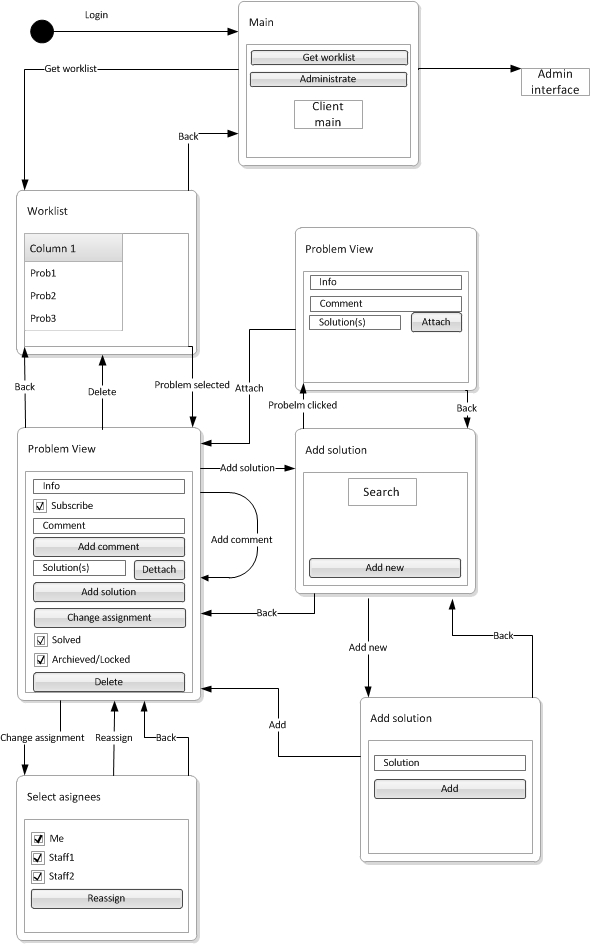
\includegraphics[width=0.90\textwidth]{input/component_design/Navigation_Diagram.jpg}
	\caption{\sinterface[c]}
	\label{fig:Navigation_Diagram}
\end{figure}


\subsubsection{\ainterface[]}

\subsection{System Interface Component}


\subsection{Function Component}


\subsection{Model Component}